\documentclass[utf8, russian, aspectratio=1610]{beamer}

\usepackage[utf8]{inputenc}
\usepackage[russian]{babel}
\usepackage{hyperref}
\usepackage{graphicx}
\usepackage{listings}
\usepackage{ucs}
\usepackage{clrscode}
\usepackage{minted}
\usepackage{clrscode}

\makeatletter
\newcommand{\minted@write@detok}[1]{%
  \immediate\write\FV@OutFile{\detokenize{#1}}}%

\newcommand{\minted@FVB@VerbatimOut}[1]{%
  \@bsphack
  \begingroup
    \FV@UseKeyValues
    \FV@DefineWhiteSpace
    \def\FV@Space{\space}%
    \FV@DefineTabOut
    %\def\FV@ProcessLine{\immediate\write\FV@OutFile}% %Old, non-Unicode version
    \let\FV@ProcessLine\minted@write@detok %Patch for Unicode
    \immediate\openout\FV@OutFile #1\relax
    \let\FV@FontScanPrep\relax
%% DG/SR modification begin - May. 18, 1998 (to avoid problems with ligatures)
    \let\@noligs\relax
%% DG/SR modification end
    \FV@Scan}
    \let\FVB@VerbatimOut\minted@FVB@VerbatimOut

\renewcommand\minted@savecode[1]{
  \immediate\openout\minted@code\jobname.pyg
  \immediate\write\minted@code{\expandafter\detokenize\expandafter{#1}}%
  \immediate\closeout\minted@code}
\makeatother

\lstset{
    extendedchars=\true,
    inputencoding=utf8x
}

\usetheme{Warsaw}
\usecolortheme{lily}
\useoutertheme[subsection=false]{smoothbars}
\useinnertheme{circles}
\setbeamertemplate{footline}[page number]{}
\setbeamertemplate{navigation symbols}{}

\renewcommand{\figurename}{} 

\title{Архитектура ЭВМ}
\subtitle{Лекция 7. Математический сопроцессор}
\author{к.ф.-м.н. Филонов Павел Владимирович \newline filonovpv@gmail.com}
\date{}


\institute[МГТУ ГА] 
{
    Московский Государственный Технический Университет \\
    Гражданской Авиации
}
\begin{document}
\begin{frame}[noframenumbering, plain]
    \titlepage
\end{frame}

\begin{frame}
    \frametitle{Содержание}
    \begin{itemize}
        \item Числа с плавающей точкой;
        \item Регистры сопроцессора;
        \item Операции:
        \begin{itemize}
            \item Обменн данными;
            \item Арифметические;
            \item Вычисление базовых функций;
        \end{itemize}
        \item Польская инверсная запись;
        \item Работа с флагами сопроцессора.
    \end{itemize}
\end{frame}

\begin{frame}
    \frametitle{Числа с плвающей точкой}

    Стандарт IEEE 754 описывает 3 формата кодирования числе с плавающей точкой:
    \begin{itemize}
        \item одинарной точности --- 4 байта;
        \item двойной точности --- 8 байт;
        \item расширенной точности --- 10 байт.
    \end{itemize}

    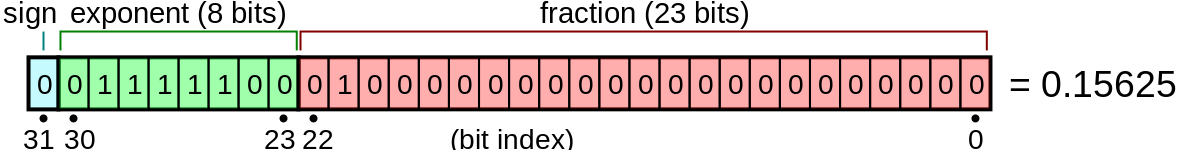
\includegraphics[width=0.75\textwidth]{fig/single.png}

    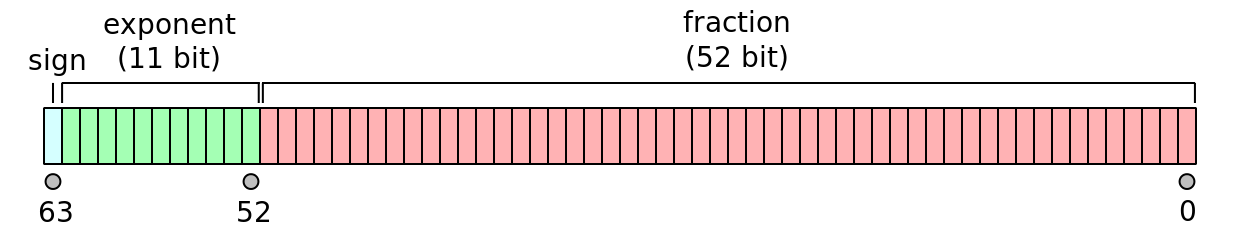
\includegraphics[width=0.8\textwidth]{fig/double.png}
    
    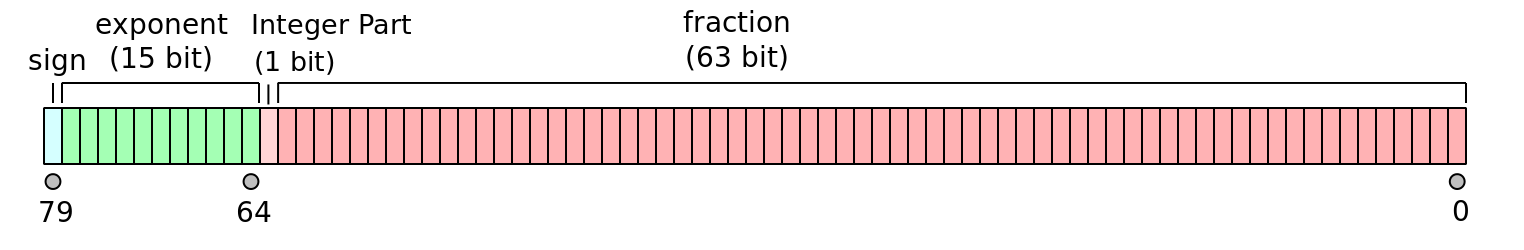
\includegraphics[width=1.0\textwidth]{fig/extended.png}


\end{frame}

\begin{frame}
    \frametitle{Регистры сопроцессора}
    \begin{figure}
        \centering
        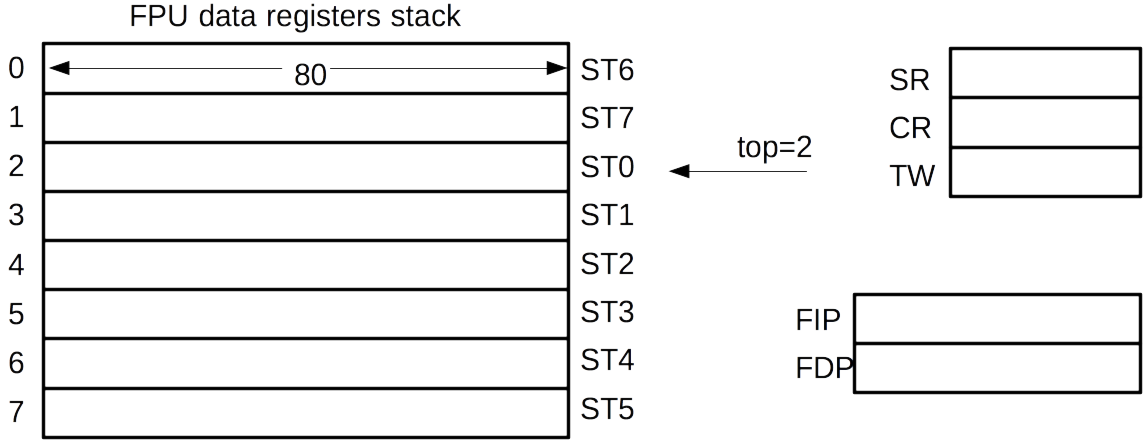
\includegraphics[width=0.95\textwidth]{fig/FPU-crop.png}
    \end{figure}
    \begin{itemize}
        \item State Register (SR)  --- регистр состояния
        \item Control Register (CR) --- регистр управления
        \item TW --- регистр тегов
        \item FIP --- хранит адрес последней выполненной сопроцессором команды
        \item FDP --- хранит аргумент последней выполненной сопроцессором команды
    \end{itemize}
\end{frame}

\begin{frame}
    \frametitle{Регистр состояния сопроцессора}
    \begin{figure}
        \centering
        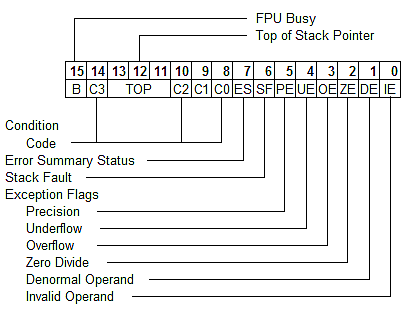
\includegraphics[width=0.75\textwidth]{fig/SR.png}
    \end{figure}
\end{frame}

\begin{frame}
    \frametitle{Обмен данными с сопроцессором}

    \begin{itemize}
        \item {\tt fld mem32/mem64/mem80/stx} --- загрузить значение на вершину стека;
        \item {\tt fst mem32/mem64/stx} --- сохранить значение с вершины стека в память или другой st регистр;
        \item {\tt fstp mem32/mem64/mem80/stx} --- тоже, что и {\tt fst}, плюс выталкивает вершину стека;
        \item {\tt fild mem16/mem32/mem64} --- загрузить в стек целое число с конвертацией в число с плавающей точкой;
        \item {\tt fist mem16/mem32} --- сохранить число с вершины стека в целочисленном формате;
        \item {\tt fistp mem16/mem32/mem64} --- тоже, что и {\tt fist}, плюс выталкиваем вершину стека;
        \item {\tt fxch} --- поменять местами {\tt st0} и {\tt st1};
        \item {\tt fxch stx} --- поменять местами {\tt st0} и {\tt stx}.
    \end{itemize}
\end{frame}

\begin{frame}
    \frametitle{Загрузка математических констант}
    Все команды загружают значение константы в регистр {\tt st0}.
    \begin{itemize}
        \item {\tt fld1} --- $1.0$;
        \item {\tt fldz} --- $+0.0$;
        \item {\tt fldpi} --- $\pi$;
        \item {\tt fld2e} --- $\log_2 e$;
        \item {\tt fld2t} --- $\log_2 10$;
        \item {\tt fldln2} --- $\ln 2$;
        \item {\tt fldlg2} --- $\lg 2$.
    \end{itemize}
\end{frame}

\begin{frame}[fragile]
    \frametitle{Пример: число $\pi$}
\begin{minted}[linenos]{nasm}
print_pi:
    push ebp
    mov ebp, esp
    sub esp, 4

    fldpi
    fstp dword [ebp - 4]
    push dword [ebp - 4]
    call print_float
    add esp, 4

    mov esp, ebp
    pop ebp
    ret
\end{minted}
\end{frame}

\begin{frame}
    \frametitle{Арифметические операции}
    \begin{itemize}
        \item {\tt fadd mem32/mem64/stx} --- прибавляет операнд к {\tt st0}
        \item {\tt fsub mem32/mem64/stx} --- вычитает операнд из {\tt st0}
        \item {\tt fsubr mem32/mem64/stx} --- вычитает {\tt st0} из операнда и сохраняет в {\tt st0}
        \item {\tt fmul mem32/mem64/stx} --- умножает операнд на {\tt st0}
        \item {\tt fdiv mem32/mem64/stx} --- делит {\tt st0} на свой операнд
        \item {\tt fdivr mem32/mem64/stx} --- делит свой операнд на {\tt st0} и сохраняет в {\tt st0}
    \end{itemize}

    Варианты над регистрами: {\tt fxxx st0, stx} или {\tt fxxx stx, st0}.

    Выталкиваюшие варианты: {\tt faddp, fsubp, fsubrp, fmulp, fdivp, fdivrp}. Работают только над регистрами
    {\tt fxxxp stx}

    Операнд --- целое число: {\tt fiadd, disub, fisubr, fimul, fidiv, fidivr}
\end{frame}

\begin{frame}
    \frametitle{Польская инверсная запись}

    Любому арифметическому выражению можно поставить в соответсвие инверсную запись, которая не будет содержать скобки.

    Примеры:
    \begin{itemize}
        \item $4 + 2 \rightarrow 4~2 +$
        \item $3*(4 + 2) \rightarrow 4~2 + 3 *$
        \item $(1 - 2)*(4 + 5) \rightarrow 1~2 - 4~5 + *$
    \end{itemize}

       \begin{codebox}
            \Procname{Алгоритм вычисления выражения в инверсной записи}
            \li \For {\bf c} $\leftarrow$ каждого элемента выражения
            \li \Do \If {\bf c} --- число
            \li     \Then push {\bf c}
            \li     \Else \If {\bf c} --- операция
            \li           \Then pop {\bf a}
            \li                 pop {\bf b}
            \li                 push применить {\bf c} к {\bf a} и {\bf b}
                          \End
                    \End
                \End
            \li pop result
            \li \Return result
        \end{codebox}
\end{frame}

\begin{frame}
    \frametitle{Пример: арифметика на стеке}

    \begin{itemize}
        \item Переведем выражение в польскую инверсную запись

            $$
            (1 - 2)*(4 + 5) \rightarrow 1~2 - 4~5 + *
            $$

        \item Используем для вычисления выражения стек
        \begin{figure}
            \centering
            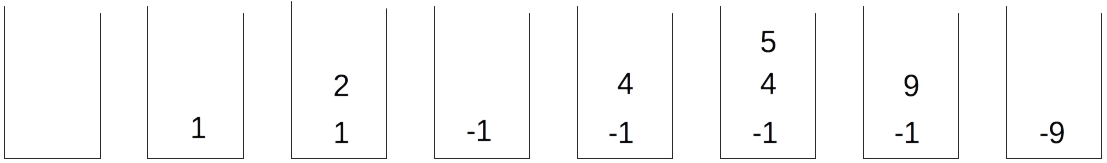
\includegraphics[width=1.0\textwidth]{fig/stack_arithm_crop.png}
        \end{figure}
    \end{itemize}
\end{frame}

\begin{frame}[fragile]
    \frametitle{Арифметика на стеке}
    $$1~2 - 4~5 + *$$
\begin{minted}[linenos]{nasm}
    fild dword [one]
    fild dword [two]
    fsubp st1
    fld dword [four]
    fld dword [five]
    faddp st1
    fmulp st1
    fstp dword [result]
    push dword [result]
    call printfloat
    add esp, 4
\end{minted}
\end{frame}

\begin{frame}[fragile]
    \frametitle{Сравнение и обработка результатов}
    Для сравнения числе с плавающей точкой испоьзуются следующие команды:
    \begin{itemize}
        \item {\tt fcom mem32/mem64/stn} --- сравнивает {\tt st0} с операндом;
        \item {\tt fcomp mem32/mem64/stn} --- тоже, что и {\tt fcmo}, плюс выталкивает {\tt st0};
        \item {\tt fcompp} --- сравнивает {\tt st0} с {\tt st1} и выталкивает оба регистра из стека. 
    \end{itemize}
    В результате работы любой из этих операций устанавливаются флаги регистра {\tt SR}. Проанализировать значение этих флагов можно скопировав их сначала в регистр {\tt ax}, а затем в {\tt FLAGS}.
\begin{minted}[linenos]{nasm}
    fstsw ax    ; сохранить SW в AX
    sahf        ; скопировать некоторые флаги из AH в FLAGS
\end{minted}

    После этой процедуры в регистр {\tt FLAGS} будут скопированы флаги {\tt ZF} и {\tt CF}. Следовательно необходимо использовать команды услвных переходов для беззнаковых чисел ({\tt ja, jb, jae, jbe, je, jne}).
\end{frame}

\begin{frame}[fragile]
    \frametitle{Пример: max}
    Напишем подпрограмму, которая возвращает максимальное из двух чисел с плавающей точкой.

\begin{minipage}[t]{0.45\linewidth}
\begin{minted}[linenos]{nasm}
max:
    push ebp
    mov ebp, esp
    sub esp, 116
    pushfd
    fsave [ebp - 116]
    finit

    fld dword [ebp + 8]
    fld dword [ebp + 12]
    fcompp
    fstsw ax
    sahf
\end{minted}
\end{minipage}
\begin{minipage}[t]{0.45\linewidth}
\begin{minted}[linenos,
               firstnumber=14]{nasm}
    ja .b_gt_a
    mov eax, [ebp + 8]
    jmp .end

.b_gt_a:
    mov eax, [ebp + 12]

.end: 
    frstor [ebp - 116]
    popfd
    mov esp, ebp
    pop ebp
    ret
\end{minted}
\end{minipage}

\end{frame}

\begin{frame}[fragile]
    \frametitle{Управление сопроцессором}

    Для управления сопроцессором используется регистр {\tt CR}.
    \begin{itemize}
        \item {\tt fstcw mem16} --- сохранить содержимое {\tt CR} в память
        \item {\tt fldcw mem16} --- загрузить значения для {\tt CR} из памяти
    \end{itemize}

    {\bf Пример:}  выставить режим округления <<в сторону нуля>>.
\begin{minted}[linenos]{nasm}
    sub esp, 2         ; выделить 2 байта на стеке
    fstcw [esp]        ; сохранить в эту область памяти значение CR
    or word [esp], 0000110000000000b
                       ; выставить биты 11 и 10 (режим округления)
    fldcw [esp]        ; загрузить новое значение CR
    add esp, 2         ; освобождаем память
\end{minted}
\end{frame}

\begin{frame}
    \frametitle{Резюме}

    \begin{itemize}
        \item форматы кодирования числе с плавающей точкой
        \begin{itemize}
            \item одинарной точности
            \item двойной
            \item расширенной
        \end{itemize}
        \item регистры сопроцессора организованы в виде стека
        \item фрифметика на стеке
        \item операции сравнения чисел с плавающей точкой
        \item управление сопроцессором осуществляется через регистр {\tt CR}
    \end{itemize}
\end{frame}
\end{document}
